\section{Implementation}

In this section, we describe the instantiation of \name on top of off-the-shelf
eventually consistent distributed store Cassandra. We particularly focus on the
challenges in realizing an efficient implementation of our model.

\begin{figure}
\begin{center}
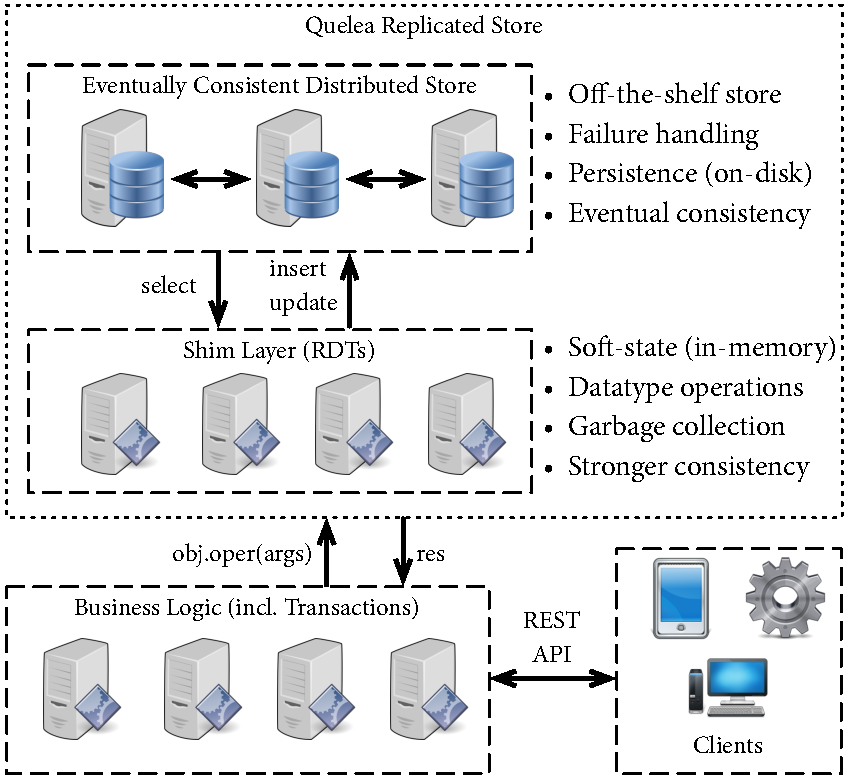
\includegraphics[width=0.9\columnwidth]{Figures/ImplModel}
\end{center}
\caption{Implementation Model.}
\label{fig:impl_mod}
\end{figure}

Figure~\ref{fig:impl_mod} describes the overall system architecture. The main
idea in our implementation of \name is to offload the majority of concerns
related to data management such as replication, fault tolerance, availability
and convergence to Cassandra, an off-the-shelf eventually consistent store
(called \emph{backing store} in the sequel). Replicated data type
implementation and the stronger consistency semantics are enforced in the
\emph{shim layer}. Our implementation supports eventual, causal and strong
consistency for operations, and RC, MAV and RR transaction semantics. All of
this functionality is implemented on top of the standard interface exposed by
Cassandra, and illustrates the portability of \name programming model. Complex
business logic is implemented with the help of transactions on the server side,
with clients interacting with the web-service over REST interface.

\subsection{Shim Layer}

The shim layer maintains a causally consistent in-memory snapshot of a subset
of objects in the backing store, by explicitly tracking dependencies introduced
between the effects due to visibility, session and same transaction relations.
The dependence tracking is similar to the techniques presented in~\cite{BoltOn}
and~\cite{Eiger}, with the usual optimizations making use of transitivity
properties for minimizing the number of dependencies. Shim layer performs the
reductions associated with replicated datatype operations corresponding to
client requests. As the backing store provides durability, convergence and
fault tolerance, each shim layer node simply acts as a soft-state cache, and
can safely be terminated at any instant. Similarly, more shim layer nodes can
be spawned on demand.

Every effect generated as a result of an effectful operation on an object
inserts a new row $(o,e,vis,txn,val)$ into the backing store, where $o$ and $e$
are object and (unique) effect identifiers, $vis$ is the set of identifiers of
effects visible to this operation, $txn$ is an optional transaction identifier,
and $val$ is the value associated with the effect. The shim layer periodically
fetches updates from the backing store for those objects which were accessed in
the previous time slice. Since causally consistent operations require an
up-to-date view of the current session, the shim layer node synchronously
fetches operations if the causally preceding operations in the current session
are not available in the cache. Strongly consistent operations are performed
after obtaining exclusive leases on objects. The lease mechanism is implemented
with the help of Cassandra's support for conditional updates and expiring
columns.
